\documentclass[12pt]{scrartcl}
\usepackage[german, ngerman]{babel}
\usepackage{graphicx}
\usepackage{color}
\usepackage{url}
\usepackage{xcolor}
\usepackage{listings}
\usepackage{hyperref}
\usepackage{nameref}
\usepackage{varioref}
\hypersetup{
    colorlinks=true,
    linkcolor={black!50!black},
    % linkcolor={red!50!black},
    citecolor={black!50!black},
    urlcolor={black!50!black}
}
\usepackage[headsepline,footsepline]{scrlayer-scrpage}
\usepackage{biblatex}
\usepackage{amsmath}
\usepackage{float}

\newcommand{\code}[1]{\texttt{#1}}


\definecolor{mGreen}{rgb}{0,0.6,0}
\definecolor{mGray}{rgb}{0.5,0.5,0.5}
\definecolor{mPurple}{rgb}{0.58,0,0.82}
\definecolor{backgroundColour}{rgb}{0.95,0.95,0.95} %{cmyk}{0.05,0.05,0.05,0.05}

\lstdefinestyle{CStyle}{
    backgroundcolor=\color{backgroundColour},
    commentstyle=\color{mGreen},
    keywordstyle=\color{blue},
    numberstyle=\tiny\color{mGray},
    stringstyle=\color{mPurple},
    basicstyle=\footnotesize,
    breakatwhitespace=false,
    breaklines=true,
    captionpos=b,
    keepspaces=true,
    numbers=left,
    numbersep=5pt,
    showspaces=false,
    showstringspaces=false,
    showtabs=false,
    tabsize=2,
    language=C++
}

\lstdefinestyle{Terminal}{
    backgroundcolor=\color{backgroundColour},
    commentstyle=\color{black},
    keywordstyle=\color{black},
    numberstyle=\tiny\color{black},
    stringstyle=\color{black},
    basicstyle=\footnotesize,
    breakatwhitespace=false,
    breaklines=true,
    captionpos=b,
    keepspaces=true,
    numbers=none,
    numbersep=5pt,
    showspaces=false,
    showstringspaces=false,
    showtabs=false,
    tabsize=2,
}


\pagestyle{scrheadings}
\clearscrheadfoot
%\cfoot{Tobias Gruber}
\cfoot{\pagemark}
\chead{\headmark}
\automark[subsection]{section}


\begin{document}


\begin{titlepage}
    \vfill
	\centering
	{\scshape\LARGE Hochschule München \par}
    {\scshape\Large Fakultät für Informatik \par}
	\vspace{1.5cm}




    \vfill
	{\LARGE\bfseries Computational Geometry\\~\\ \par}
	{\LARGE\bfseries Praktikumsaufgabe 1\par}
	\vfill
    \vfill


    \begin{tabular}{ll}
    \normalsize
    Team:  & Christopher Hinz, Tobias Gruber\\
    \end{tabular}

	\vfill

\end{titlepage}

\newpage



\raggedright


\section{Problemstellung}
In dem Tar-File 'strecken.tgz' (s.u.) befinden sich Dateien mit jeweils 4 Koordinaten pro Zeile.
Diese stellen jeweils die x- und y-Koordinaten eines Start- bzw. Endpunkts einer Strecke dar.
Die Datei soll eingelesen und die Anzahl der sich schneidenden Strecken durch paarweises Testen herausgefunden werden.
Zusätzlich wird die pro Datei aufgewendete Zeit gemessen.
Es ist zu begründen, warum die Anzahl der vom Programm jeweils gefundenen Schnittpunkte korrekt ist.

\section{Vorüberlegung}

Um einschätzen zu können inwiefern die Ergebnisse sinnvoll sind sollen an dieser Stelle einige Vorüberlegungen getroffen werden.\\~\\
Welche Anzahl an Schnitten sind zu erwarten bzw. in welchem Wertebereich sollten sich die Ergebnisse bewegen?\\
Die minimal zu erwartende Anzahl an Schnitten wäre für 1.000, 10.0000 und 100.000 Strecken jeweils null.
Dies ist somit die untere Grenze des zu erwartenden Wertebereichs.
Die maximale Anzahl an Schnitten würden in dem Fall auftreten, dass sich alle Strecken gegenseitig schneiden.
Dann wäre nämlich für jede Strecke ein Schnittpunkt mit allen anderen Strecken gegeben.
Das Problem ist in der Mathematik auch als Sektglasproblem bekannt.
Die Berechnung erfolgt in Anlehnung an die Formel für die Dreieckszahlen.
Für eine Anzahl von n Strecken ergeben sich somit k Schnittpunkte wie folgt:
\begin{equation}
k = \frac{(n-1) \cdot n}{2}
\end{equation}
Damit wären für 1.000 Strecken maximal $499.500$ (für 10.000 maximal $49.995.000$,
für 100.000 maximal $4.999.950.000$) zu erwarten.
Dies ist somit die obere Grenze des zu erwartenden Wertebereichs.

\section{Umsetzung}

\subsection{Umsetzung der Aufgabenstellung}

Das Programm verwendet die Funktion \code{read\_dat()} um die Daten aus den Dateien einzulesen und über \code{pack\_koords()} die Datensätze zu Strecken zusammenzufassen.
Jede Strecke wird anschließend gegen alle anderen Strecken geprüft, ob sie diese schneidet, oder nicht.
Zur Feststellung, ob sich die zwei Strecken schneiden wird ausgewertet, ob die Punkte $p_1, p_2$ der ersten Strecke zu den Punkten $p_1, p_2$ der zweiten Strecke im oder gegen den Uhrzeigersinn angeornet sind.
Dafür wird folgende Formel verwendet, die im Ergebnis den Betrag des Kreuzproduktes aus den Richtungsvektoren der drei Punkte enthält:
\begin{equation}
    ccw(p, q, r) := \begin{vmatrix} p_1 & p_2 & 1 \\ q_1 & q_2 & 1 \\ r_1 & r_2 & 1 \end{vmatrix} = (p_1q_2 - p_2q_1) + (q_1r_2 - q_2r_1) + (p_2r_1 - p_1r_2)
\end{equation}

Ist das Prdukt der ccw-Funktion der ersten Strecke mit den Endpunkten der zweiten Strecke, sowie das Produkt der ccw-Funktion der zweiten Strecke mit den Endpunkten der ersten Strecke kleiner oder gleich 0, so kann unter der Annahme, dass die Strecken nicht kollinear zueinander sind davon ausgegangen werden, dass sich die Strecken schneiden.

Sind die Strecken Kollinear angeordnet, so ergeben beide Kreuzprodukte 0. In diesem Fall muss noch überprüft werden, ob sich die Strecken überlappen.
Bei Überlappung der Strecken lässt sich mindestens einer der Endpunkte der zweiten Strecke über ein Vielfaches zwischen 0 und 1 des ersten Streckenvektors addiert mit einem Endpunkt der ersten Strecke darstellen.
Da zuvor bereits festgestellt wurde, dass die Strecken kollinear sind, kann das Skalar zum Richtungsvektor der zweiten Strecke über das Auflösen der parametrischen Darstellung durch die x-Komponenten der Orstvektoren aufgelöst werden.
\begin{equation}
    \lambda = \frac{x_r - x_p}{x_q - x_p}
\end{equation}
Liegt der Wert von $\lambda$ zwischen 0 und 1, so überlappen sich die Funktionen. Nimmt $\lambda$ den Wert 0 oder 1 an, schneiden sich die Strecken in in jeweils einem der Enpunkte.

\begin{lstlisting}[style=CStyle, caption={p1\_lib.h: Bibliotheksfunktionen},captionpos=b]
#include <fstream>
#include <iostream>
#include <string>
#include <vector>


struct point{
    float x;
    float y;
};

struct line{
    point p1;
    point p2;
};


void read_dat(char* filename, unsigned int N, std::vector<float>& v){
    std::ifstream file;
    file.open(filename);
    float data;
    for(int i = 0; i < N; ++i){
        file >> data;
        v.push_back(data);
    }
    file.close();
}


void pack_koords(std::vector<float>& source, std::vector<line>& target){
    line temp;
    for(unsigned int i = 0; i < source.size()/4; ++i){
        temp.p1.x = source[0+i];
        temp.p1.y = source[1+i];
        temp.p2.x = source[2+i];
        temp.p2.y = source[3+i];
        target.push_back(temp);
    }
}

float ccw(point p, point q, point r){
    float res = (p.x*q.y - p.y*q.x)+ (q.x*r.y - q.y*r.x) + (p.y*r.x  - p.x*r.y);
    return res;
}

bool line_intersect_check(line l1, line l2){
    bool retval = false;
    float ccw_res1 = ccw(l1.p1, l1.p2, l2.p1) * ccw(l1.p1, l1.p2, l2.p2);
    float ccw_res2 = ccw(l2.p1, l2.p2, l1.p1) * ccw(l2.p1, l2.p2, l1.p2);
    if(ccw_res1 <= 0.0f && ccw_res2 <= 0.0f){
        retval = true;
        if(ccw_res1 == 0.0f && ccw_res2 == 0.0f){
            float lambda1 = (l1.p1.x-l2.p1.x)/(l2.p2.x-l2.p1.x);
            float lambda2 = (l1.p2.x-l2.p1.x)/(l2.p2.x-l2.p1.x);
            if ((lambda1 < 0 || lambda1 > 1) && (lambda2 < 0 || lambda2 > 1)) retval = false;
        }
    }
    return retval;
}
\end{lstlisting}



\begin{lstlisting}[style=CStyle, caption={strecken.cpp: Aufgruf der Bibliotheksfunktionen},captionpos=b]
#include "p1_lib.h"
#include <chrono>


int main(){
    auto start = std::chrono::steady_clock::now();


    std::vector<float> vec;
    std::vector<line> lines_vec;
    read_dat((char*)"strecken/s_1000_1.dat", 1000, vec);
    pack_koords(vec, lines_vec);


    int intersect_counter = 0;
    for(unsigned int i = 0; i < lines_vec.size(); ++i){
        for(unsigned int j = 0; j < lines_vec.size(); ++j){
            if(i!=j){
                if(line_intersect_check(lines_vec[i], lines_vec[j])){
                    ++intersect_counter;
                }
            }
        }
    }

    std::cout << "Strecken insgesamt: " << vec.size() << "\n" << "Schnitte zweier Strecken: " << intersect_counter << "\n";

    auto end = std::chrono::steady_clock::now();
    std::cout << "Runtime: "
    << (float)std::chrono::duration_cast<std::chrono::microseconds>(end - start).count()/1000
        + std::chrono::duration_cast<std::chrono::milliseconds>(end - start).count() << " ms\n";

    return 0;
}
\end{lstlisting}

In \autoref{lst:ausgabe_strecken} wird die Ausgabe des Programmes zur Schnittpunktezählung aufgeführt.
In der Ausgabe ist zu erkennen, dass die Anzahl der Schnitte für alle Fälle (1.000, 10.000, 100.000) im zu erwartenden Wertebereich liegt.
Schnittpunkte:
\begin{itemize}
    \item 1.000 Strecken: $0<= 62.250 <= 499.500$
    \item 10.000 Strecken: $0<= 6.247.500 <= 49.995.000$
    \item 100.000 Strecken: $0<= 624.975.000 <= 4.999.950.000$
\end{itemize}


\begin{lstlisting}[style=Terminal, caption={testing.cpp: Ausgabe Konsole},captionpos=b, label={lst:ausgabe_strecken}]
# s_1000_1.dat
Strecken insgesamt: 1000
Schnitte zweier Strecken: 62250
Runtime: 14.408 ms
#s_10000_1.dat
Strecken insgesamt: 10000
Schnitte zweier Strecken: 6247500
Runtime: 580.073 ms
#s_100000_1.dat
Strecken insgesamt: 100000
Schnitte zweier Strecken: 624975000
Runtime: 55100.2 ms
\end{lstlisting}


\subsection{Programm zum Testen der Funktion}
Um die korrekte Funktionsweise des Programmes zu verifizieren werden verschiedene Testfälle definiert.
Die Testfälle decken unterschiedliche Streckenanordnungen ab und sollen dadurch die in der Vorlesung besprochenen Grenzfälle für Streckenschnitte überprüfen.
\autoref{fig:test_cases} zeigt die implementierten Testfälle.

\begin{figure}[ht]
    \graphicspath{ {./pictures/} }
    \centering
    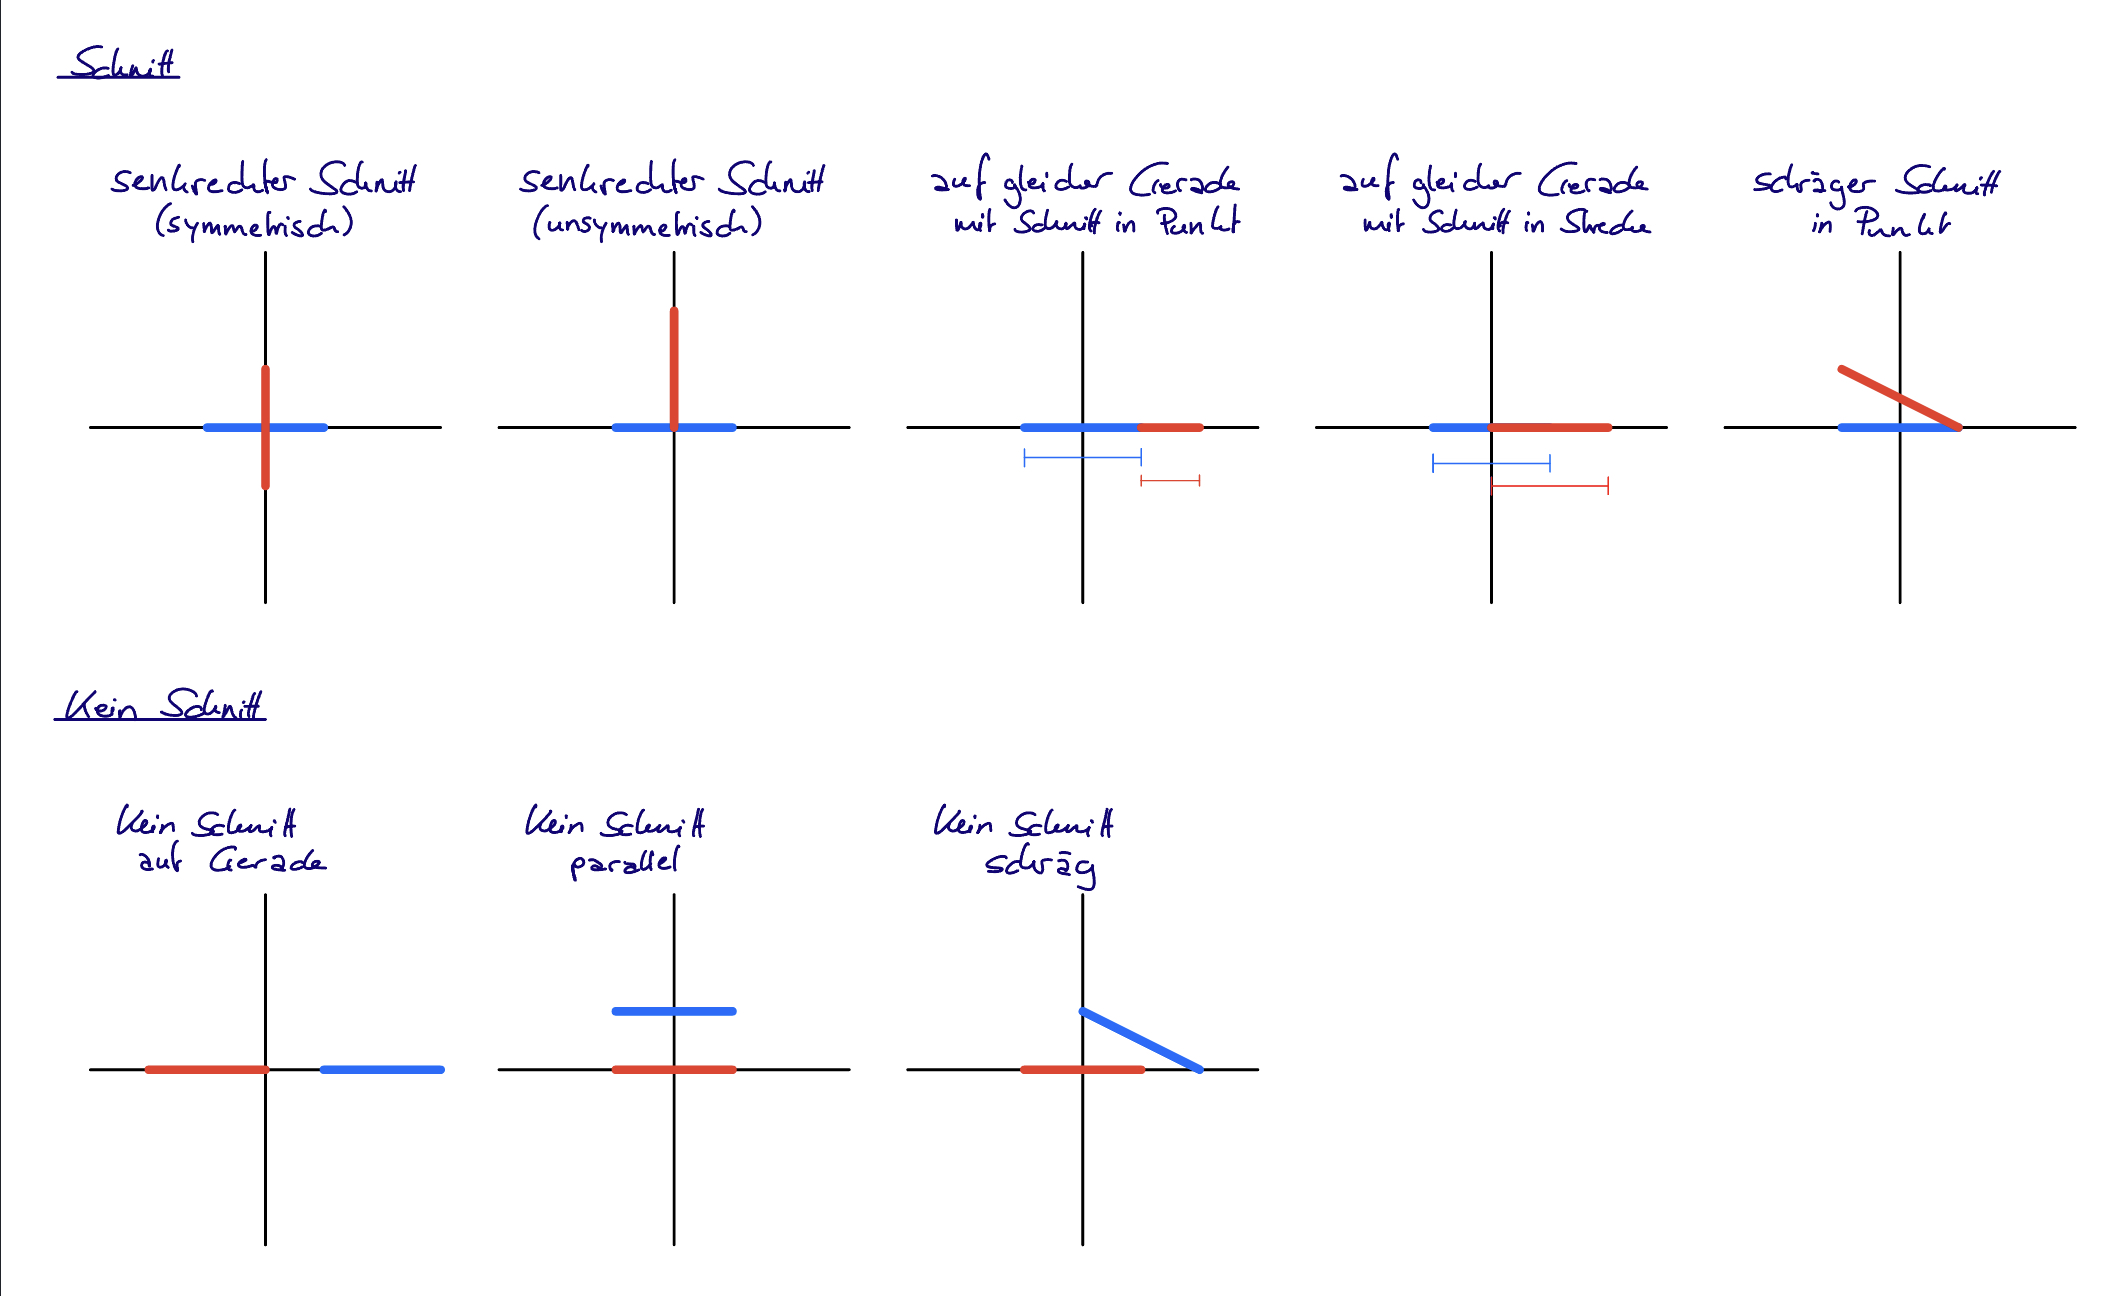
\includegraphics[scale=0.2]{Test_Vorlage.jpeg}
    \smallskip
    \caption{Testfälle für Streckenschnitte}
    \label{fig:test_cases}
\end{figure}

\autoref{lst:test_code} zeigt die Implementierung der Testfälle in C++.\\

\begin{lstlisting}[style=CStyle, caption={testing.cpp: Testen der Bibliotheksfunktionen},captionpos=b, label={lst:test_code}]
#include "p1_lib.h"

void print_result(line l1, line l2, bool b_soll){
    std::cout << std::boolalpha << "Soll: " << b_soll << ", Ist: " << line_intersect_check(l1, l2) << "\n";
}


int main(){

    // Verschiedene Schnitte

    // Strecken mit senkrechtem Schnitt (symmetrisch)
    // p1 = (0,1) nach p2 = (0,-1)
    // p1 = (1,0) nach p2 = (-1,0
    print_result(line{.p1.x = 0, .p1.y = 1, .p2.x = 0, .p2.y = -1}, line{.p1.x = 1, .p1.y = 0, .p2.x = -1, .p2.y = 0}, true);

    // Strecken mit senkrechtem Schnitt (unsymmetrisch)
    // p1 = (0,2) nach p2 = (0,0)
    // p1 = (1,0) nach p2 = (-1,0)
    print_result(line{.p1.x = 0, .p1.y = 2, .p2.x = 0, .p2.y = 0}, line{.p1.x = 1, .p1.y = 0, .p2.x = -1, .p2.y = 0}, true);

    // Strecken auf gleicher Gerade mit Schnitt in einem Punkt
    // p1 = (1,0) nach p2 = (2,0)
    // p1 = (1,0) nach p2 = (-1,0)
    print_result(line{.p1.x = 1, .p1.y = 0, .p2.x = 2, .p2.y = 0}, line{.p1.x = 1, .p1.y = 0, .p2.x = -1, .p2.y = 0}, true);

    // Strecken auf gleicher Gerade mit Schnitt in einer Strecke
    // p1 = (0,0) nach p2 = (2,0)
    // p1 = (1,0) nach p2 = (-1,0)
    print_result(line{.p1.x = 0, .p1.y = 0, .p2.x = 2, .p2.y = 0}, line{.p1.x = 1, .p1.y = 0, .p2.x = -1, .p2.y = 0}, true);

    // Strecken auf gleicher Gerade mit Schnitt in einer Strecke
    // p1 = (0,0) nach p2 = (2,0)
    // p1 = (1,0) nach p2 = (-1,0)
    print_result(line{.p1.x = 1, .p1.y = 0, .p2.x = -1, .p2.y = 1}, line{.p1.x = 1, .p1.y = 0, .p2.x = -1, .p2.y = 0}, true);


    // Verschiedene ohne Schnitt

    // Strecken ohne Schnitt auf Gerade
    // p1 = (-2,0) nach p2 = (0,0)
    // p1 = (1,0) nach p2 = (3,0)
    print_result(line{.p1.x = -2, .p1.y = 0, .p2.x = 0, .p2.y = 0}, line{.p1.x = 1, .p1.y = 0, .p2.x = 3, .p2.y = 0}, false);

    // Strecken ohne Schnitt parallel
    // p1 = (-2,0) nach p2 = (0,0)
    // p1 = (-2,1) nach p2 = (0,2)
    print_result(line{.p1.x = -2, .p1.y = 0, .p2.x = 0, .p2.y = 0}, line{.p1.x = -2, .p1.y = 1, .p2.x = 0, .p2.y = 2}, false);

    // Strecken ohne Schnitt schraeg
    // p1 = (-2,0) nach p2 = (0,0)
    // p1 = (0,1) nach p2 = (2,0)
    print_result(line{.p1.x = -2, .p1.y = 0, .p2.x = 0, .p2.y = 0}, line{.p1.x = 0, .p1.y = 1, .p2.x = 2, .p2.y = 0}, false);

    return 0;
}
\end{lstlisting}

\ \\~\\
\autoref{lst:ausgabe_test} zeigt, dass für die Testfälle die erwarteten Ergebnisse erzielt werden.
Das bedeutet, dass für alle Streckenpaare, die wie in den Testfällen angeordnet sind, die Schnittstellenfunktion korrekt berechnet ob sie sich schneiden oder nicht.\\

\begin{lstlisting}[style=Terminal, caption={testing.cpp: Ausgabe Konsole},captionpos=b, label={lst:ausgabe_test}]
Soll: true, Ist: true
Soll: true, Ist: true
Soll: true, Ist: true
Soll: true, Ist: true
Soll: true, Ist: true
Soll: false, Ist: false
Soll: false, Ist: false
Soll: false, Ist: false
\end{lstlisting}


\end{document}
